\setchapterimage[6cm]{chapter/spacecraft/Takhir-Salakhov-For-You-Humanity-1961-2011-title-moved.jpg}

\setchapterpreamble[u]{\margintoc}
\chapter{Spacecraft and space stations}
\labch{spacecraft}
\footnotetext{Painting by Takhir Salakhov ``For You, Humanity!'' (1961), reproduced on the stamp of Azerbaijan in 2011 on the 50th anniversary of First Manned Space Flight (the flight of Yuri Gagarin). 
\href{https://commons.wikimedia.org/wiki/File:Stamps\_of\_Azerbaijan,\_2011-944.jpg}{Wikimedia Commons}.}

The chapter is devoted to research of spaceships and stations based on Wikidata. 
Using SPARQL scripts, a list of Russian ships and stations is constructed, 
a timeline of the launching of ships in our country and in the world for the period from 1960 to 2021 is drawn. 
An evaluation of the completeness of Wikidata was performed, showing, 
that many of the items have the wrong value of the property 
\wdProperty{31}{instance of}. In the course of the work, it was found that the current performance of Russian astronautics in terms of the number of spacecraft launches in recent years matches that of the USSR fifty years ago. 

\section{List of space ships and stations}
Let's build a query~\ref{lst:spaceships} to output a list of all spaceships and stations. 
We need the objects \wdqName{space station}{25956}, 
\wdqName{spacecraft}{40218} and the relation \wdProperty{31}{instance of}. 

\index{SPARQL!VALUES!List of space ships and stations}
\index{SPARQL!SERVICE!List of space ships and stations}
\begin{lstlisting}[ language=SPARQL, breaklines=true, numbers=none,%
                    caption={Retrieves list of all spaceships and stations. The result contained \num{145} objects in 2021. SPARQL query: \href{https://w.wiki/4eeL}{https://w.wiki/4eeL}},%
                    label=lst:spaceships,%
                    texcl%
                    ]
# List of spacecraft (Q40218) and space station (Q25956)
SELECT  ?s ?sLabel ?typeLabel
WHERE
{
  VALUES ?type {wd:Q40218 wd:Q25956}
  ?s wdt:P31 ?type.  # Selecting the type of object
  SERVICE wikibase:label {bd:serviceParam wikibase:language"en"}
}
\end{lstlisting}%

\begin{marginfigure}
{
	\setlength{\fboxsep}{0pt}%
	\setlength{\fboxrule}{1pt}%
	\fcolorbox{gray}{gray}{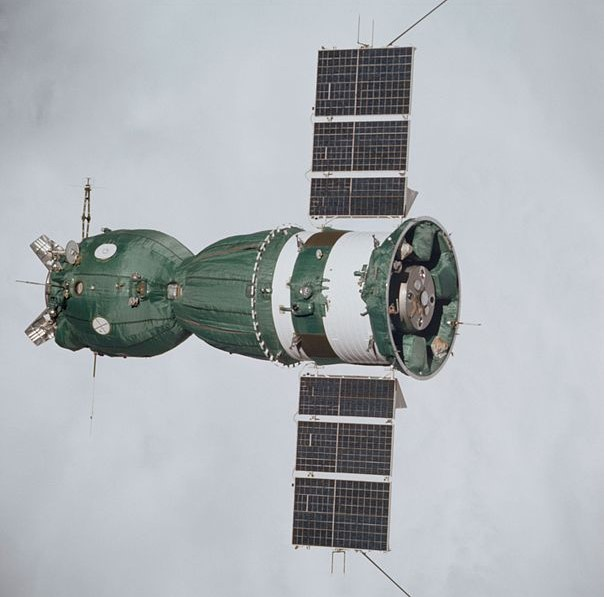
\includegraphics{graphics/chapter/spacecraft/soyuz-19.jpg}}
}
\caption[Soyuz-19.]%
{In which country is the machine shown in the picture designed?
See the answer~\ref{answer:spacecraft_USSR} on the p.~\pageref{answer:spacecraft_USSR}.}
\label{question:spacecraft_soyuz19}
\end{marginfigure}

\section{Depth of object development}

As of 2021 on Wikidata \wdqName{Apollo-8}{184201} {wdqName} is the most complete and elaborate spacecraft, which has 30 properties.\autocite{spacecraftProWD} At the same time, only one property each has ships such as: \wdqName{Europa Astrobiology Lander}{10491365}, \wdqName{Project Orbiter}{6514453}, \wdqName{LRK}{5961734}, \wdqName{EarthForce One}{5327028}%
\sidenote[][]{%
Note the difficult fate of the object \wdqName{EarthForce One}{5327028}. This object was automatically created in Wikidata by a bot in 2013, because there was an English Wikipedia article. According to the ``\href{https://en.wikipedia.org/wiki/EarthForce_One}{EarthForce One}`` English Wikipedia, the article was removed due to a lack of reliable sources proving the significance of the site. And the object has been left as an unremarkable item on Wikidata. Think of a query that would output a list of similar Wikidata items, that does not match any Wikipedia article.%
},%
\wdqName{Souyz GVC}{60767924}, %
\wdqName{CubeSat for Solar Particles}{22907583}.\autocite{spacecraftProWD} %
To find this information, a query built with the ProWD\autocite{spacecraftProWD} service was used. %
The same service showed that the number of properties of space objects is uneven, %
most are less than 30\% filled.\autocite{spacecraftProWD} %

\section{List of Soviet and Russian spaceships and stations}

Let us find ships and stations designed in USSR or Russia, using the query~\ref{lst:spaceshipsUSSR}.

\index{SPARQL!VALUES!List of Soviet and Russian spaceships and stations}
\index{SPARQL!SERVICE!List of Soviet and Russian spaceships and stations}
\begin{lstlisting}[ language=SPARQL, breaklines=true, numbers=none,%
                    caption={Retrieves list of Soviet and Russian spaceships and stations. \num{3} results in 2017 and \num{25} results in 2021. SPARQL query: \href{https://w.wiki/4eeR}{https://w.wiki/4eeR}},%
                    label=lst:spaceshipsUSSR,%
                    texcl%
                    ]
# List of Russian and USSR spacecrafts and stations
SELECT  ?spacecraft  ?spacecraftLabel 
WHERE
{
  {?spacecraft wdt:P31 wd:Q40218.} UNION #spacecraft
  {?spacecraft wdt:P31 wd:Q25956.} # and space station
  
  # Soviet Union and Russia
  VALUES ?ruCountries {wd:Q15180 wd:Q159}
  ?spacecraft wdt:P17 ?ruCountries. # related to Russia
  
  SERVICE wikibase:label {bd:serviceParam wikibase:language "en"}
}
\end{lstlisting}%

\begin{marginfigure}
{
	\setlength{\fboxsep}{0pt}%
	\setlength{\fboxrule}{1pt}%
	\fcolorbox{gray}{gray}{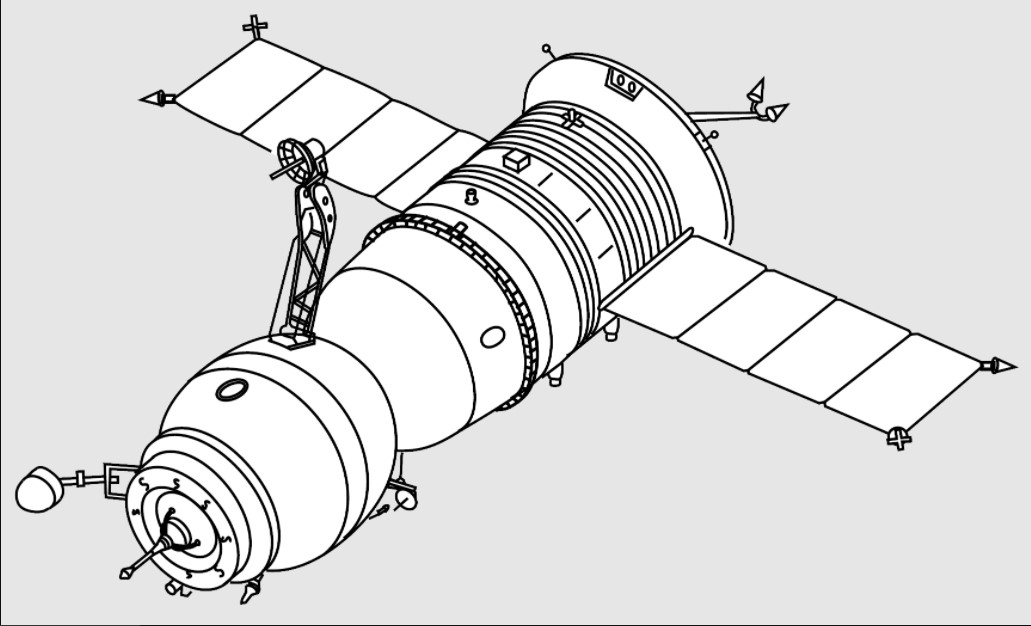
\includegraphics{graphics/chapter/spacecraft/soyuz-t.jpg}}
}
\caption
[Soyuz-T.]{%
In which country is the machine shown in the picture designed?

See the answer~\ref{answer:spacecraft_USSR} on the p.~\pageref{answer:spacecraft_USSR}.
}
\label{question:spacecraft_soyuzT}
\end{marginfigure}

\section{Analyzing the Completeness of Wikidata}

Let us analyze the degree of filling in Wikidata in the field of Soviet and Russian spaceships and stations.
By Query~\ref{lst:spaceships} 145 results were obtained for all ships and stations,
by Query~\ref{lst:spaceshipsUSSR} about Soviet and Russian objects~--- only 25.
Information about~Soviet and Russian objects in 2021
has become several times more compared to 2017,
when on Query~\ref{lst:spaceshipsUSSR} only 3 objects were returned.

As of 2021, the Buran.ru website in the section about the spaceships of the USSR and Russia contains information about 36 ships.\autocite{spacecraftBuran} %
There are 51 launches of spaceships from 1957 to 1984 in Soviet Union and 43 in same years in the United States.\autocite[480-483]{spacecraftCosmonavtika} This means that less than half of the Soviet spaceships are represented in Wikidata.
There are 10 Soviet and Russian launches of space stations\autocite[296]{spacecraftSAA},
126 NASA shuttle launches from 1981 to 2008\autocite[288]{spacecraftSAA}
and 31 international launch vehicles\autocite[290-291]{spacecraftSAA} in the American directory of space and astronomy.

\section{Time schedules of space exploration in Russia (include USSR) and the World}

Spacecraft launch schedule in Russia since 1960s (Figure~\ref{fig:launchesRussia5years})
built with Query~\ref{lst:launchesRussia5years}.%

Earlier, in queries to get any lists, we used the \wdProperty{31}{instance of} property.
The Query~\ref{lst:launchesRussia5years} without this property, with using the relation
\wdProperty{619}{<< spaceship launch date >>} on line 10
for traversing and counting such objects that have been launched into space.
%
%%%%%%%%%%%%%%%% Exercise 1 %%%%%%%%%%%%%%%% 
\label{question:spacecraft_1}%
\marginnote{%
How many ships were launched in the~USSR in the~1960s, 1970s, and 1980s? %
See answer~\ref{answer:launches_USSR} on p.~\pageref{answer:launches_USSR}.%
}%
%
The logical operator \lstinline|UNION| on lines 5-8 in Query~\ref{lst:launchesRussia5years}
allows you to combine Soviet and Russian spacecraft launches.

If in the Query~\ref{lst:launchesRussia5years} instead of the variable \lstinline|?Lapse|~---\lstinline|?year| remained (lines 3 and 12),
then we would get in Figure~\ref{fig:launchesRussia5years}
the number of launches each year.
Thanks to the rounding function \lstinline|FLOOR()|
and grouping%
\sidenote[][8.0cm]{
%
On line 14 of the query,~\ref{lst:launchesRussia5years}
objects launched into space are grouped by the command:
\mbox {\lstinline|GROUP BY ?lapse|.} \newline
The fact that the grouping goes exactly according to five-year range, and not, for example, six-year-olds,
is defined on line 12, where the \lstinline|?year| divided by 5, rounded, and multiplied by 5.%
%
},
\lstinline|?item| objects that have launches are grouped over a five-year period,
and into the variable \lstinline|?quantity| the number of these objects is recorded,
calculated using the \lstinline|COUNT()| function.

The BarChart command in Query~\ref{lst:launchesRussia5years} is used to present the results as a bar chart in Figure~\ref{fig:launchesRussia5years}.

\index{SPARQL!STR!Schedule of spacecraft launches in the USSR and Russia (by five years)}
\index{SPARQL!COUNT!Schedule of spacecraft launches in the USSR and Russia (by five years)}
\index{SPARQL!UNION!Schedule of spacecraft launches in the USSR and Russia (by five years)}
\index{SPARQL!BarChart!Schedule of spacecraft launches in the USSR and Russia (by five years)}
\index{SPARQL!GROUP BY!Schedule of spacecraft launches in the USSR and Russia (by five years)}
\index{SPARQL!ORDER BY!Schedule of spacecraft launches in the USSR and Russia (by five years)}
\index{SPARQL!BIND!Schedule of spacecraft launches in the USSR and Russia (by five years)}
\index{SPARQL!FLOOR!Schedule of spacecraft launches in the USSR and Russia (by five years)}
\begin{lstlisting}[ language=SPARQL, breaklines=true, %
                    caption={Draw schedule of spacecraft launches in the USSR and Russia (by five years). Found \num{14} five-year plans in 2021. SPARQL query: \href{https://w.wiki/4f7Y}{https://w.wiki/4f7Y}},%
                    label=lst:launchesRussia5years,%
                    texcl%
                    ]
# The number of spacecraft launches in Russia every 5 years
#defaultView:BarChart
SELECT (STR(?lapse) AS ?lapse_str) (COUNT(?item) AS ?quantity)
WHERE {                                  # spacecraft belongs to
        {?item wdt:P17 wd:Q15180}               # country = USSR
  UNION {?item wdt:P17 wd:Q159}               # country = Russia
  UNION {?item wdt:P495 wd:Q159}    # country of origin = Russia
  UNION {?item wdt:P495 wd:Q15180}.  # country of origin =  USSR
  
  ?item wdt:P619 ?launch. # date of spacecraft launch
  BIND( YEAR(?launch) AS ?year) 
  BIND(FLOOR(?year/5)*5 AS ?lapse) # count for each 5 years
} 
GROUP BY ?lapse
ORDER BY ?lapse # Order 1970, 1975, 1980, ...
\end{lstlisting}%

\index{Graph!Diagram!Schedule of spacecraft launches in the USSR and Russia (by five years)}
\begin{figure*}[h!]
  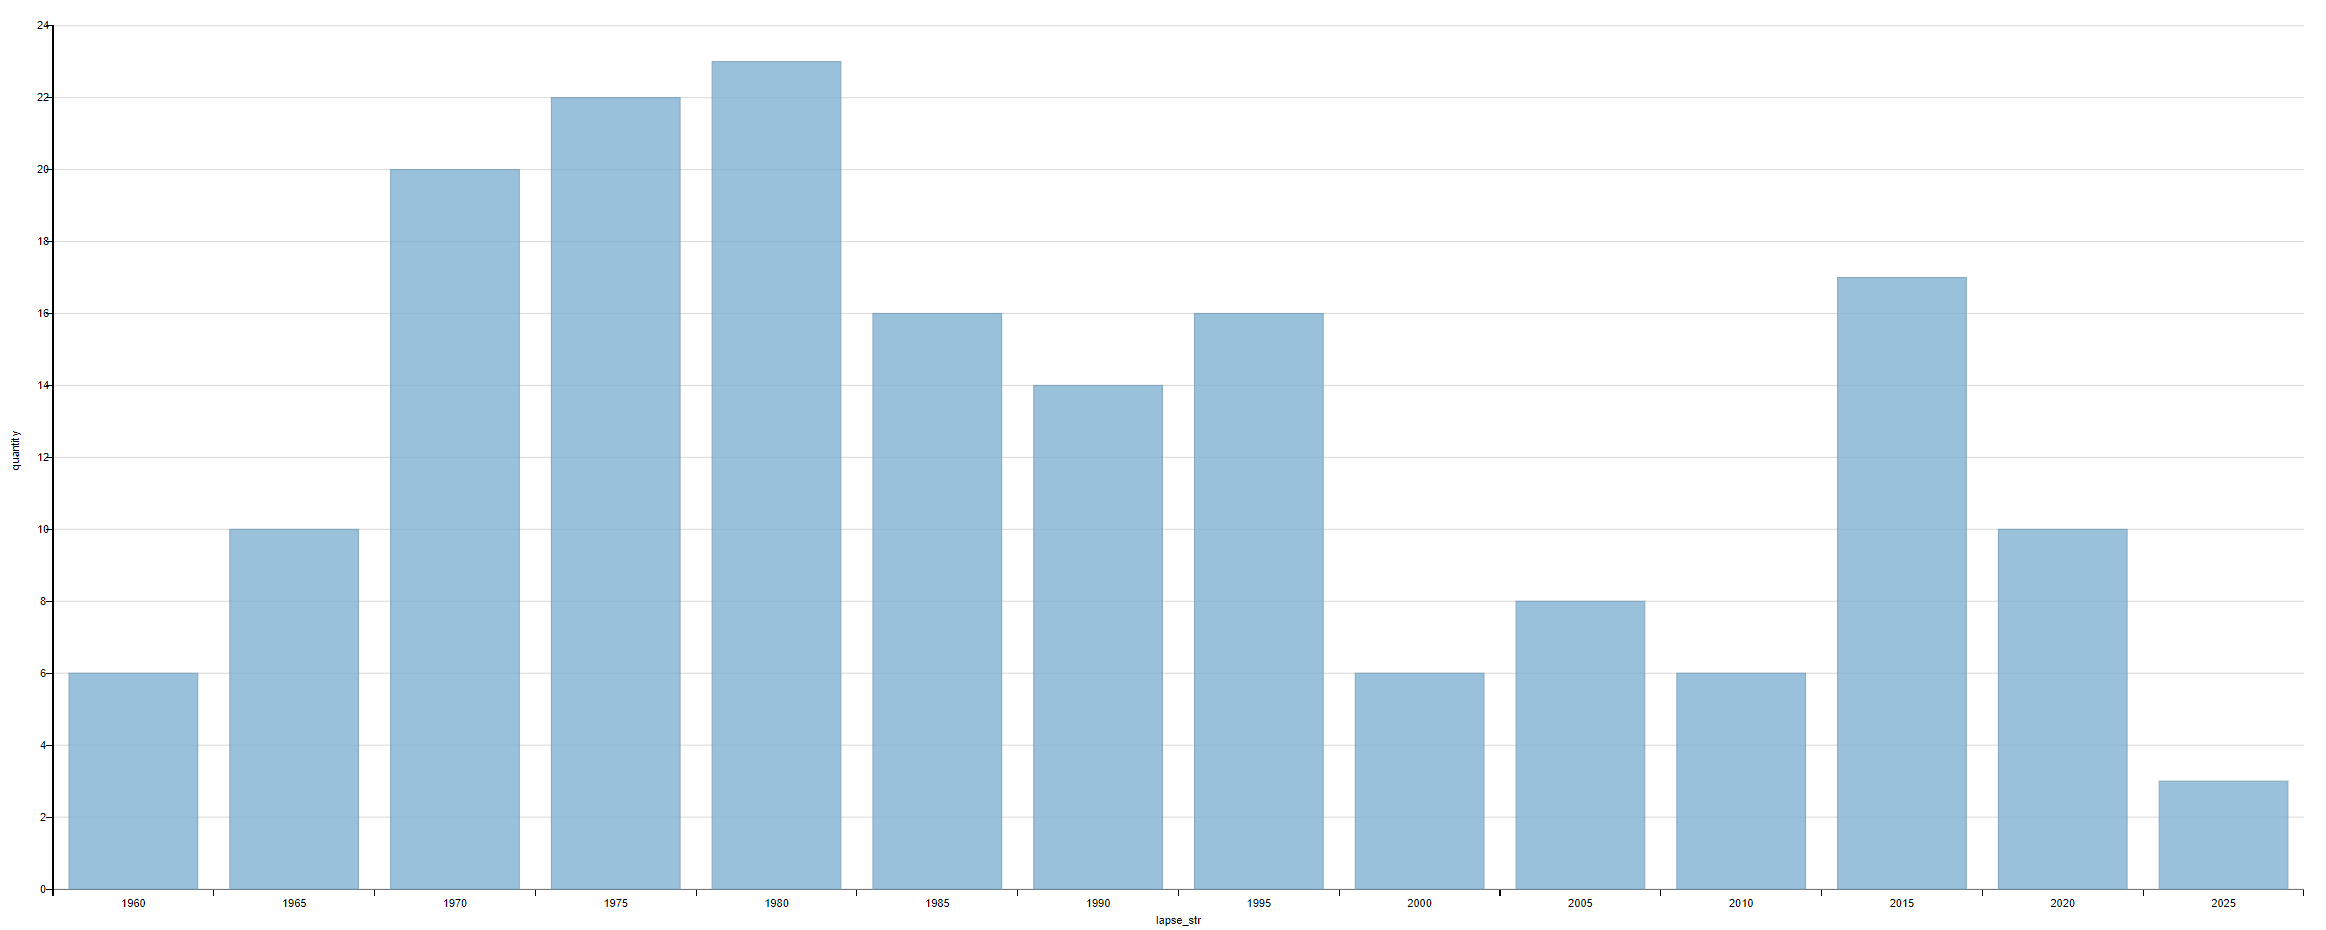
\includegraphics[width=\linewidth]{graphics/chapter/spacecraft/Visualization of the number of spacecraft launches in USSR and Russia per 5 years 2022.png}
  \caption[Schedule of spacecraft launches in the USSR and Russia (by five years)] {Visualization of the number of spacecraft launches in the USSR and Russia every 5 years, built with Query~\protect\ref{lst:launchesRussia5years}, 2022.}%
  \label{fig:launchesRussia5years}%
\end{figure*}

The horizontal axis in Figure~\ref{fig:launchesRussia5years} is answered by the variable \mbox{\lstinline|?lapse_str|}. 
If you don't convert the number \lstinline|?lapse| 
into a text variable \mbox{\lstinline|?lapse_str|}%
\sidenote[][]{
%
Converting a number into text  
in the third line of the query~\ref{lst:launchesRussia5years}:\newline
\lstinline|(STR(?lapse) AS ?lapse_str)|.%
%
}, then the~X axis has a range from 0 to 2200, 
instead of the required range from 1960 to 2025, 
and the results are indicated by points with coordinates (five years, number of launches), 
and the graph becomes unreadable. 

The Figure~\ref{fig:launchesRussia5years} shows, 
that the most active period of Russian cosmonautics development was in 1970--1995.

The Query~\ref{lst:launchesWorld} draws Figure~\ref{fig:launchesWorld} 
of spacecraft launches in the World by year and country.

\index{SPARQL!STR!Diagram of the number of spacecraft launches by year and country}
\index{SPARQL!BIND!Diagram of the number of spacecraft launches by year and country}
\index{SPARQL!COUNT!Diagram of the number of spacecraft launches by year and country}
\index{SPARQL!SERVICE!Diagram of the number of spacecraft launches by year and country}
\index{SPARQL!GROUP BY!Diagram of the number of spacecraft launches by year and country}
\index{SPARQL!YEAR!Diagram of the number of spacecraft launches by year and country}
\begin{lstlisting}[ language=SPARQL, breaklines=true, %
                    caption={Draws a diagram of the number of spacecraft launches by year and country. \num{328} results in 2021. SPARQL query: \href{https://w.wiki/4f8v}{https://w.wiki/4f8v}},%
                    label=lst:launchesWorld,%
                    texcl%
                    ]
# Diagram of spacecraft launches by year and country
#defaultView:BarChart
SELECT ?year (COUNT(?obj) AS ?count) ?country ?countryLabel
WHERE {
  ?obj wdt:P17 ?country. # spacecraft belongs to country 
  ?obj wdt:P619 ?launch. # date of spacecraft launch
  BIND(STR(YEAR(?launch)) AS ?year)
  
SERVICE wikibase:label {bd:serviceParam wikibase:language"en"}
}
GROUP BY ?year ?country ?countryLabel
\end{lstlisting}%

\index{Graph!Diagram!The schedule of spacecraft launches worldwide by year and country}
\begin{figure*}[h!]
  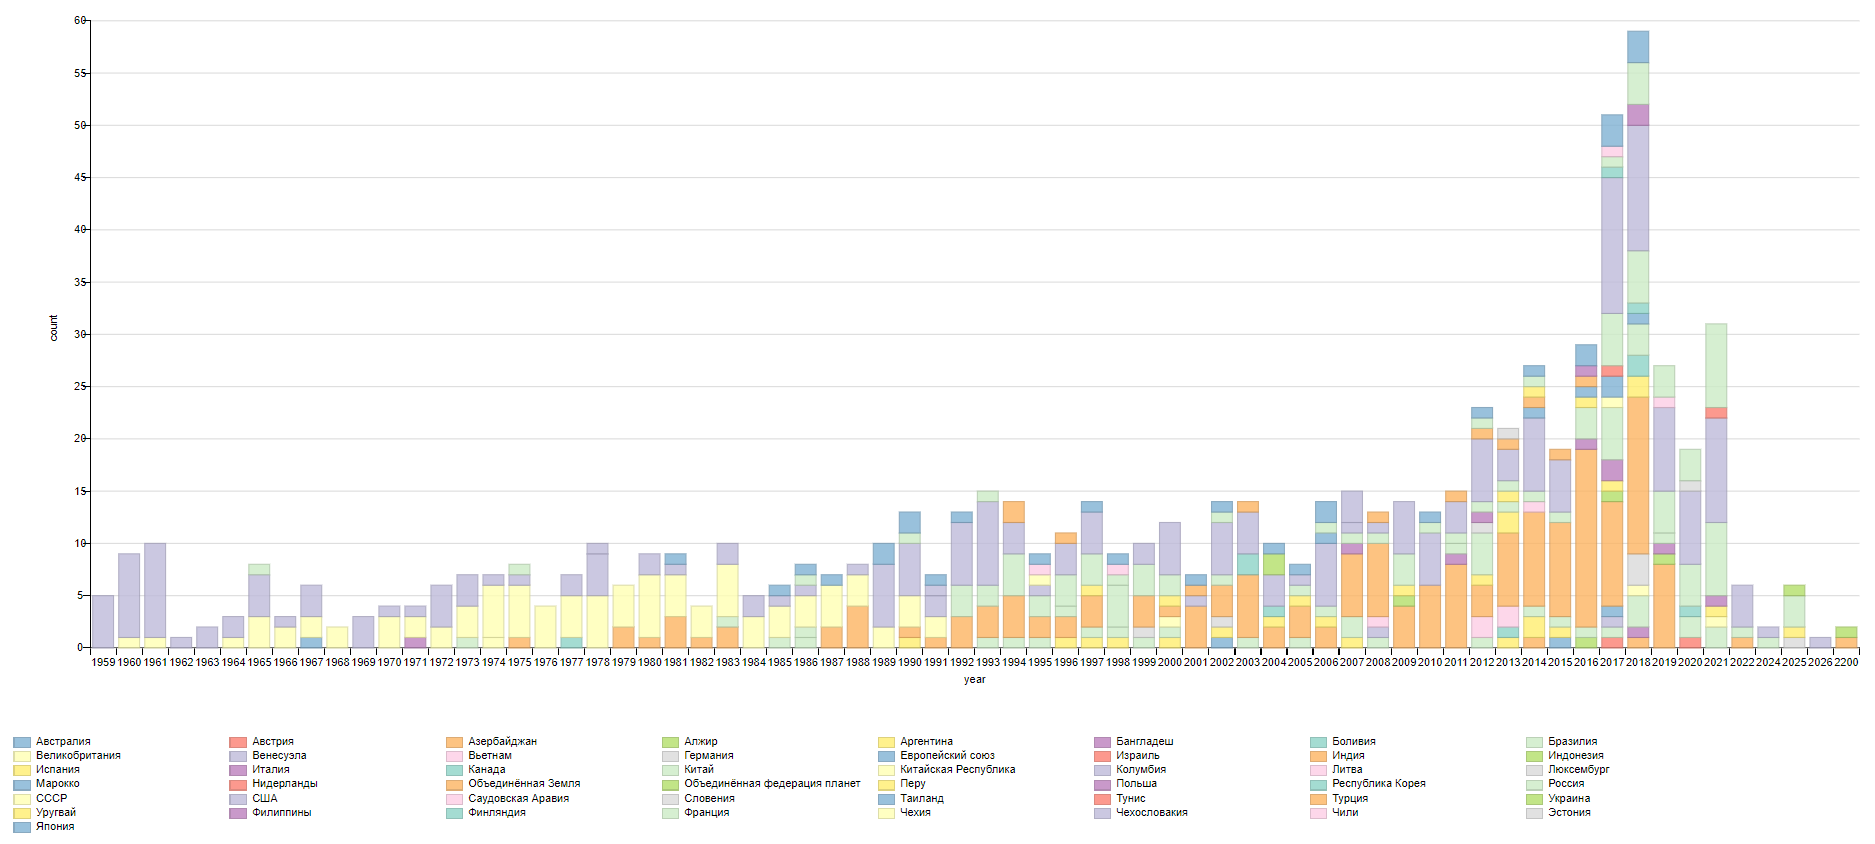
\includegraphics[width=\linewidth]{graphics/chapter/spacecraft/Visualization of the number of spacecraft launches by year and country 2021.png}
  \caption[The schedule of spacecraft launches worldwide by year and country]{Visualization of the number of spacecraft launches by year and country, built using a Query~\protect\ref{lst:launchesWorld} in 2021.}
  \label{fig:launchesWorld}%
\end{figure*}

Figure~\ref{fig:launchesWorld} shows that the most spacecraft 
launched by India and the United States. 
(only they launched more than 10 annual launches) in 2017--2018. 
Worldwide launches peaked in 2018 (59 launches). 

According to Wikidata, Russian cosmonautics ranks average in the number of launches, 
its numbers for 2016--2019 are similar to those of the USSR in the 1970s and 1980s 
and about 3--5 launches per year.

%%%%%%%%%%%%%%%% Exercise 2 %%%%%%%%%%%%%%%% 
\label{question:spacecraft_2}
\marginnote{%
What was the highest and lowest number of spacecraft launches humanity made in a decade between 1970 and 2010?
See answer~\ref{answer:max-min-space-launches} on p.~\pageref{answer:max-min-space-launches}.
}

\section{Astronauts in international flights}

Query~\ref{lst:internationalFlights} builds a graph~\ref{fig:internationalFlights} with vertices corresponding ``spaceships`` and ``astronaut``, colored by country.

\index{SPARQL!BIND!Draw the graph with the vertices of the type ``spaceships`` and ``astronauts`` with coloring by country.}
\index{SPARQL!SERVICE!Draw the graph with the vertices of the type ``spaceships`` and ``astronauts`` with coloring by country.}
\index{SPARQL!VALUES!Draw the graph with the vertices of the type ``spaceships`` and ``astronauts`` with coloring by country.}
\begin{lstlisting}[ language=SPARQL, breaklines=true, %
                    caption={Draw the graph with the vertices of the type ``spaceships`` and ``astronauts`` with coloring by country. The result contained \num{68} objects in 2022. SPARQL query: \href{https://clck.ru/agMjd}{https://clck.ru/agMjd}},%
                    label=lst:internationalFlights,%
                    texcl%
                    ]
# Graph of astronauts as crew of flights of different countries
#defaultView:Graph
SELECT DISTINCT ?item ?itemLabel ?rgb ?link ?naut_seed
WHERE
{ 
  VALUES ?toggle { true false }
  # Let's select a subset of astronauts
  {
    SELECT DISTINCT ?naut WHERE
    { 
      VALUES ?naut_seed {wd:Q313815}.  # Sergei Krikalev
      ?s wdt:P1029 ?naut_seed, ?naut;  
    }       # ?naut seed and ?naut are member of a same crew
  }
  ?s  wdt:P31/wdt:P279* wd:Q40218; # spacecraft
      wdt:P31/wdt:P279* wd:Q752783;# human spaceflight
          wdt:P1029 ?naut;  # has member of the crew ?naut    
  SERVICE wikibase:label {bd:serviceParam wikibase:language "en"}
  BIND(IF(?toggle,?s,?naut) AS ?item).
  BIND(IF(?toggle,?sLabel,?nautLabel) AS ?itemLabel).
  BIND(IF(?toggle,"FFFFFF","7FFF00") AS ?rgb_source).
  BIND(IF(?toggle,"",?s) AS ?link).
  ?naut wdt:P27 ?country. # astronaut is citizen of country 
  # ?toggle = true then spacecraft node
  # ?toggle = false then astronaut node
  BIND(     # Soviet and Russian astronauts have red nodes
    IF(!?toggle && (?country=wd:Q15180||?country=wd:Q159),"FF0000",
    IF(!?toggle && ?country=wd:Q30,"FF00FF",  # USA - fuchsia
    IF(!?toggle && ?country=wd:Q183,"C0C0C0", # Germany - silver
    IF(!?toggle && ?country=wd:Q142,"008080", # France - teal
    IF(!?toggle && ?country=wd:Q40,"800000", # Austria - maroon
    IF(!?toggle && ?country=wd:Q38,"00FFFF", # Italy - aqua
    ?rgb_source))))))
    AS ?rgb).
}
\end{lstlisting}%

\begin{marginfigure}
{
	\setlength{\fboxsep}{0pt}%
	\setlength{\fboxrule}{1pt}%
	\fcolorbox{gray}{gray}{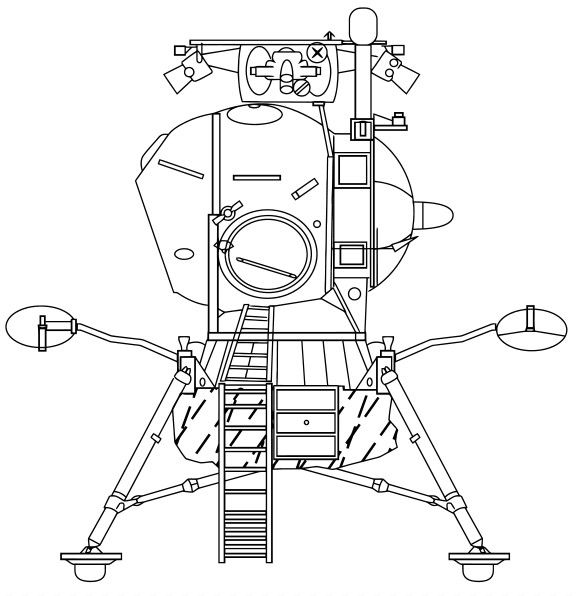
\includegraphics{graphics/chapter/spacecraft/lunar_landler.jpg}}
}
\caption[Lunar lander.]{%
In which country is the machine shown in the picture designed?

See the answer~\ref{answer:spacecraft_USSR} on the p.~\pageref{answer:spacecraft_USSR}.}
\label{question:spacecraft_lunar}
\end{marginfigure}

For the Query~\ref{lst:internationalFlights} to work, you must specify the starting point~--- an astronaut who has participated in the international spaceflight. The starting point is set at line 11 of the Query~\ref{lst:internationalFlights} and written to the \mbox{\lstinline|?naut_seed|} variable. Next, at line 12, we search for astronauts who have flown with the one we specified earlier. Lines 15--17 load data about spacecraft, flights and astronauts. Boolean variable \lstinline|?toggle| has value \lstinline|?true| if the found object is a spacecraft or \lstinline|?false| if the found object is an astronaut. The selected object (spacecraft or astronaut) is written to the \lstinline|?item| variable in line 19. In line 20 the name of the object is written to the variable \lstinline|?itemLabel|, in line 21 the data for the coloring of ships is written to the variable \mbox{\lstinline|?rgb_source|}. 

If a ship is selected, then nothing is written to the variable \lstinline|?link| in line 22. If an astronaut is selected, then his ship is written to the variable~\lstinline|?link|. On the graph this variable will correspond to the arc from the astronaut to the ship. 

Line 23 loads the astronaut's citizenship data, and~ lines 26--34 assign a color to the vertices of the astronauts in the graph, depending on their citizenship. 

\index{Graph!Graph!The graph with the vertices of the type ``spaceships`` and ``astronauts`` with coloring by country}
\begin{figure*}[h]
  \setlength{\fboxsep}{0pt}%
  \setlength{\fboxrule}{1pt}%
  \fcolorbox{gray}{gray}{%
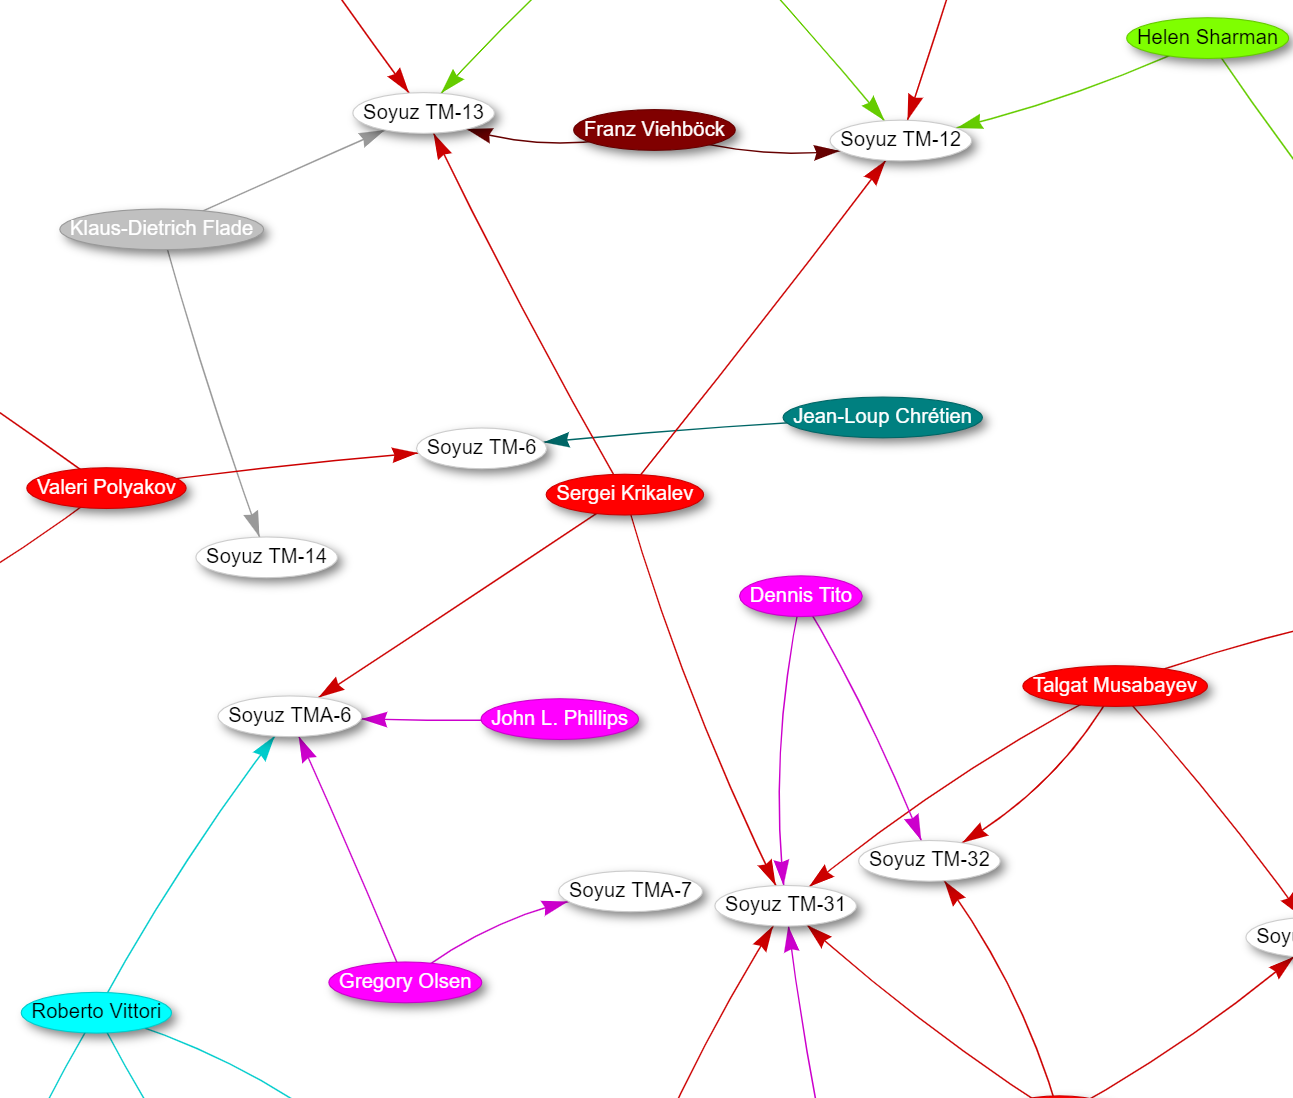
\includegraphics[width=\linewidth]{graphics/chapter/spacecraft/Cosmonauts in international flights EN.png}}
  \caption[The graph with the vertices of the type ``spaceships`` and ``astronauts`` with coloring by country]{The graph with the vertices of the type ``spaceships`` and ``astronauts`` with coloring by country. Red corresponds to the USSR and Russia, fuchsia~--- the USA, silver~--- Germany, teal~--- France, maroon~--- Australia, and aqua~--- Italy. The graph is built with the Query~\protect\ref{lst:internationalFlights}, 2022.}
  \label{fig:internationalFlights}%
\end{figure*}

\section{Exercises}
\begin{enumerate}
  \item Construct a list of ships that reached or will go to \wdqName{Mars}{111}.
  \item Calculate the proportion of ships (draw a graph by decade) which were sent 
        sent to \wdqName{Mars}{111} 
        in relation to the number of ships sent to \wdqName{Mars}{405}.
  \item Count the number of \wdqName{successful}{7632586} space launches 
      vis-a-vis \wdqName{failure}{1121708}\sidenote[][-32pt]{%
%
For example, the object \wdqName{<<Luna programme>>}{192372} 
the property \wdProperty{793}{<<significant event>>} 
specifies the number of successful and unsuccessful launches.%
}.%
\end{enumerate}
